%%%% SEITENRAENDER, SCHRIFTGROESSE UND ZEILENABSTAND NICHT ABAENDERN => SONST GIBT ES PUNKTEABZUG
\documentclass[a4paper,11pt,singlespacing]{article}
% \usepackage[left=2.5cm,right=2.5cm,top=2.5cm]{geometry}
\usepackage{setspace}
\usepackage[utf8]{inputenc}
\usepackage[T1]{fontenc}
\usepackage{graphicx}
\usepackage[ngerman]{babel}
\usepackage{color}
\usepackage{wrapfig}
\usepackage{titleref}
\usepackage{hyperref}
\usepackage[rightcaption]{sidecap}
\usepackage{listings,xcolor}
\usepackage[numbers,round]{natbib}
\usepackage{float} % For image floating ([H] -> "here")

% Configuration
\sloppy
\setlength{\parindent}{0ex} % Absatzeinrückung verhindern
\graphicspath{ {images/} }

\begin{document}
\pagenumbering{roman}

% Cover
\title{Systemadministration - Mailserver Honeypot zum analysieren von Spam}
\author{Manuel Adams 27470, Michael Ruf 27428, Mario Waizenegger 29608}
\maketitle
\begin{abstract}
Heutzutage wird viel \nameref{itm:Spam} verschickt. Einiges davon wird erkannt und gefiltert.
Um die Analyse von Spam-Nachrichten und deren Versender zu ermöglichen, wird ein Mailserver \nameref{itm:Honeypot} aufgesetzt.
Dieser soll \nameref{itm:Spam}-Nachrichten erhalten können, sowie als offener Verteiler für Spammer verfügbar sein.
\end{abstract}

\newpage

% Table of contents
\tableofcontents

\newpage
\pagenumbering{arabic}

% Content
\section{Einleitung}\label{sec:Einleitung}
	% "Wir" erlaubt
	Warum \nameref{itm:Spam} versandt wird ist vielen Menschen ein Rätsel.
	Das wirft die Fragen auf, wer Spam versendet und was die Beweggründe von Spammern sind.
	Wie geht man mit Spam um und was passiert wenn man auf \nameref{itm:Spam} reagiert?
	Ein \nameref{itm:Spam} \nameref{itm:Honeypot} bietet die Möglichkeit diese Fragen zu analysieren und die nötigen Daten zu erheben.
	% NOTE Warum lohnt sich das?
	\\
	Da die Methoden von erfolgreichen Spammern nicht dokumentiert sind, ist das Bekanntmachen des "`\nameref{itm:OpenRelay}"'"~Servers schwierig.
	Zudem ist es zeitaufwendig die eigenen Mail-Adressen unter Spammern bekannt zu machen und viele authentische Spam-Mails in kurzer Zeit zu erhalten eine Herausforderung.
	% NOTE Man kann man beim Ergebnis nochmal Stellungnahme hierzu nehmen oder den Text hier ergänzen
	% -----
	% - Wirtschaftlichkeit
	% - Andere Beweggründe
	% - Findet man Informationen über Systeme, von denen Spam verschickt wird?
	% - Werden die Nachrichten generiert? (Bots)

	\subsection{Ziel der Arbeit}\label{sec:EinleitungZiel}
		Es soll durch einen Mailserver Honeypot Erkenntnisse über Herkunft, Zweck und Zielgruppe von \nameref{itm:Spam} Nachrichten erhalten werden.
		Zusätzlich soll erarbeitet werden welche weiteren nützlichen Informationen man den Mails entnehmen kann.
		Durch diese Informationen soll die Motivation von Spammern besser verstanden und entsprechende Vorkehrungen zum Schutz ermöglicht werden.
		% NOTE Was wird genau analysiert
	
	\subsection{Vorgehensweise}\label{sec:EinleitungVorgehensweise}
		Um den Honeypot zu realisieren muss der Mail-Dienst aus dem Internet zugänglich sein.
		Dieser besteht hierbei aus Ausgangsserver und Eingangsserver.
		Hierzu werden auf einer \nameref{itm:VirtuelleMaschine} die Dienste in \nameref{itm:Container}n aufgesetzt.
		Aus Sicherheitsgründen muss die VM ins interne Netz abgeschottet sein.
		Der Aufbau ist in \autoref{fig:Hierarchy} visualisiert.

		% TODO Schrift vom Bild viel zu klein
		\begin{figure}[H]
		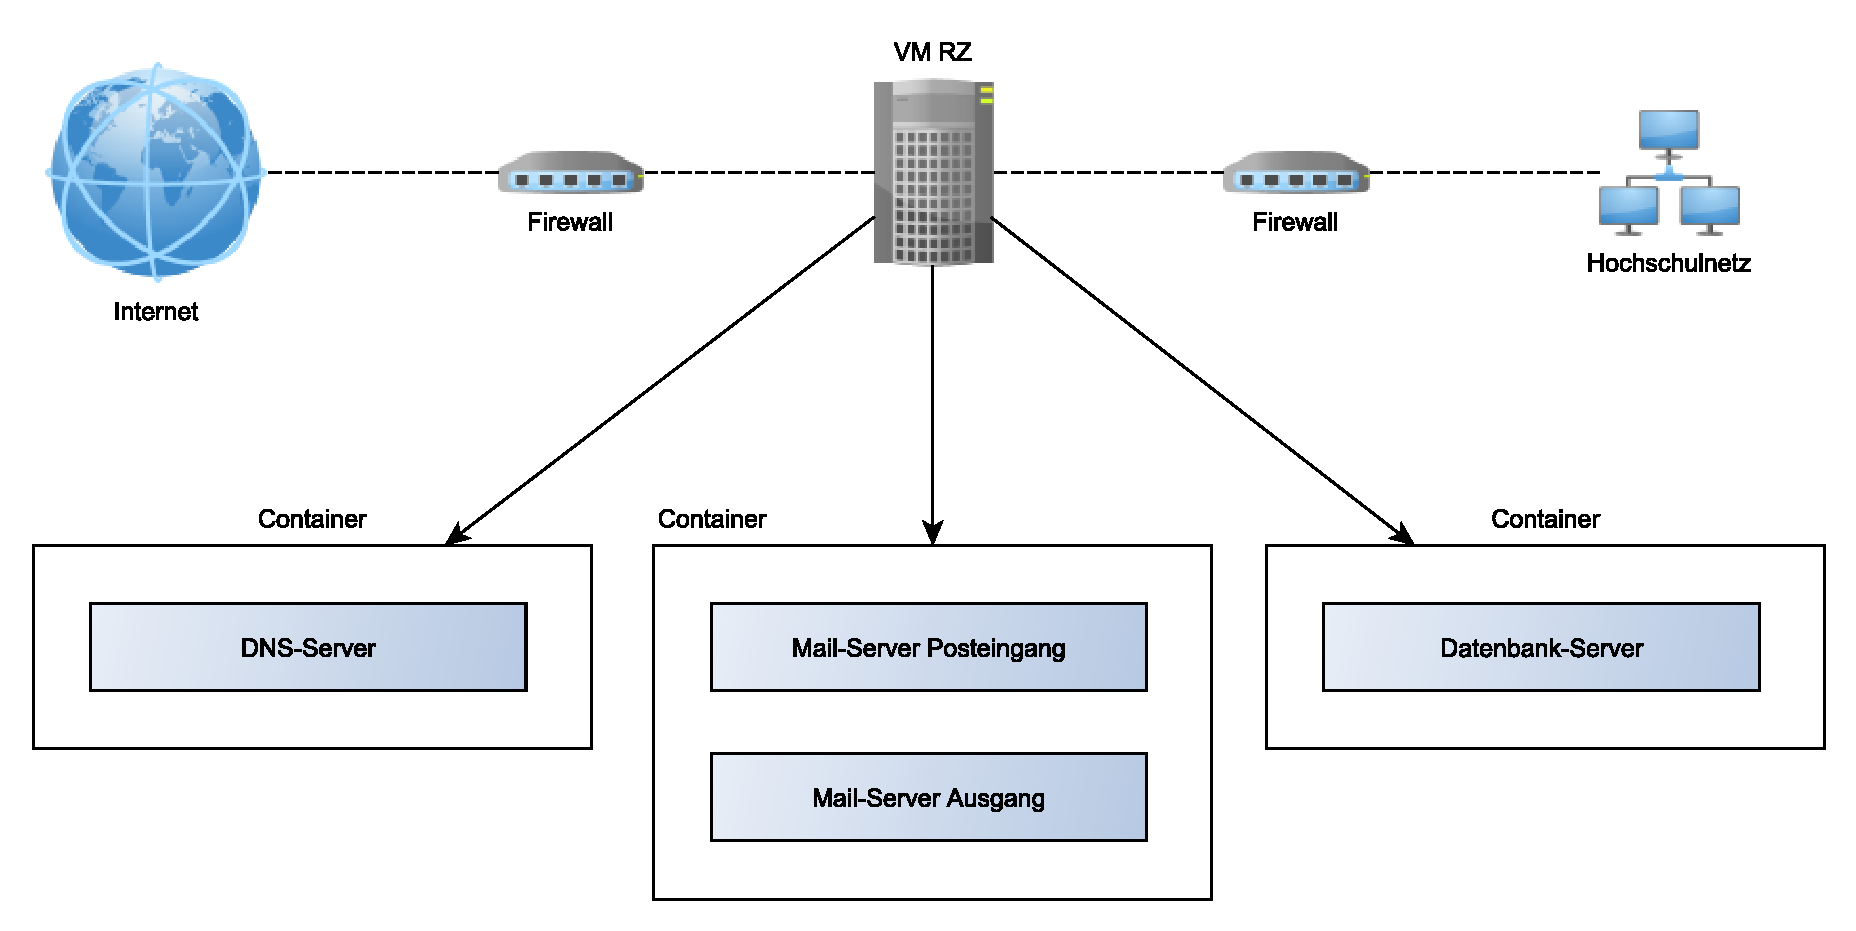
\includegraphics[width=\linewidth]{2-Hierarchy.png}
		\caption{Netzwerkstruktur}
		\label{fig:Hierarchy}
		\end{figure}

		Um den Eingangsserver zu realisieren sind folgende Aufgaben erforderlich:
		\begin{enumerate}
		\item Mail Eingangsserver bereitstellen und konfigurieren
		\item \nameref{itm:DNS} Server einrichten um realistische E-Mail-Adressen bereitzustellen
		\item Bei möglichst vielen Diensten mit unterschiedlichen Mailadressen registrieren
		\item Mails analysieren
		\end{enumerate}

		Den Ausgangsserver betreffend sind folgende Aufgaben erforderlich:
		\begin{enumerate}
		\item Mail Ausgangsserver bereitstellen und konfigurieren
		\item Als "`\nameref{itm:OpenRelay}"' im Internet durchsickern lassen
		\item Eingehende Mails tatsächlich weiterleiten
		\item Mails analysieren
		\end{enumerate}

%	\subsection{Aufbau der Arbeit}\label{sec:EinleitungAufbau}
%		% Hier geht es wirklich um den Aufbau der wissenschaftlichen Arbeit, nicht um das Projekt
%		In Abschnitt 2 geht es um..
%		In Abschnitt 3 geht es um..
%		TODO


\section{Grundbegriffe}\label{sec:Grundbegriffe}
	Die folgenden Begriffsdefinitionen und Unterscheidungen sind zum einen zur Verdeutlichung, wie Begriffe in dieser Arbeit verstanden werden und um Fachbegriffe zu erklären.
	
	% NOTE Alle nochmal durchnudeln
	\begin{description}
	\item[Spam\label{itm:Spam}]\hfill \\
		Als Spam oder Junk werden unerwünschte, in der Regel auf elektronischem Weg übertragene Nachrichten (Informationen) bezeichnet, die dem Empfänger unverlangt zugestellt werden und häufig werbenden Inhalt enthalten. Dieser Vorgang wird Spamming oder Spammen genannt, der Verursacher Spammer.\cite{Spam}
	\item[Honeypot\label{itm:Honeypot}]\hfill \\
		Sicherheitstechnisch scheinbar verwundbares Computerprogramm, das Computerviren, -würmer und Trojaner anlockt, um sie zu registrieren und unschädlich zu machen.\cite{Honeypot}
	\item[Open Relay\label{itm:OpenRelay}]\hfill \\
		Ein SMTP-Relay-Server der durch unzureichende Sicherheitskonfiguration auch Mails weiterleitet bei denen er weder für die Absender- noch für die Zieladresse zuständig ist, wird als "`Open relay"' bezeichnet.\cite{SMTP-Relay-Server}
	\item[Virtuelle Maschine (VM)\label{itm:VirtuelleMaschine}]\hfill \\
		Eine VM ist eine Kapselung eines Rechnersystems auf Softwareebene. Dadurch lässt sich eine Rechnerarchitektur in einem Container simulieren. \cite{VM}
	\item[Blacklist \label{itm:Blacklist}]\hfill \\
		Eine Blacklist oder "`schwarze Liste"' enthält eine Auflistung von Daten, die von einem Prozess ausgeschlossen werden solle. Das Gegenteil dazu ist eine Whitelist. \cite{Blacklist}
	\item[Container\label{itm:Container}]\hfill \\
		Containervirtualisierung ist eine Methode, um mehrere Instanzen eines Betriebssystems isoliert voneinander auf einem Hostsystem zu betreiben.\cite{Container}
	\item[DNS\label{itm:DNS}]\hfill \\
		Das Domain Name System (DNS) ist einer der wichtigsten Dienste in vielen IP-basierten Netzwerken. Seine Hauptaufgabe ist die Beantwortung von Anfragen zur Namensauflösung.\cite{DNS}
	\item[DKIM\label{itm:DKIM}]\hfill \\
		DKIM (DomainKeys Identified Mail) ist eine Methode der E-Mail-Authentifizierung. DKIM fügt Ihren Mails eine Signatur hinzu, die Ihrer Domain zugeordnet ist und bei allen ausgehenden E-Mails genutzt wird. Das Verwenden eines DomainKey ist eine Technik (ähnlich wie SPF), die das Fälschen des Absenders einer E-Mail erschweren soll.\cite{DKIM}
	\item[Hook\label{itm:Hook}]\hfill \\
		Hook (englisch für Haken, auch Einschubmethode genannt) bezeichnet in der Programmierung eine Schnittstelle, mit der fremder Programmcode in eine bestehende Anwendung integriert werden kann, um diese zu erweitern, deren Ablauf zu verändern oder um bestimmte Ereignisse abzufangen.\cite{Hook}
	\item[Catch-All-Mail-Adressen\label{itm:Catch-All-Mail}]\hfill \\
		Ein Catch-All-e-Mail-Konto ist eine Adresse, die alle Nachrichten mehr erhalten möchten, die an eine falsche e-Mail-Adresse für eine Domain adressiert sind angegeben ist.\cite{Catch-All-Mail}
	\end{description}


\section{Problemstellung}\label{sec:Problemstellung}
	% Hier erstmal noch zusammen fassen

	% Unterpunkte:
	% - Sehr konkret
	% - Forschungsfrage festnageln

	\subsection{Konfiguration}\label{sec:ProblemstellungKonfiguration}
		Um einen reibungslosen Ablauf zu gewährleisten muss der Mailserver in der Lage sein Mails zu empfangen und zu senden.
		Die Authentizität des Mailservers gegenüber anderen wird über verschiedene Mechanismen wie bspw. "`\nameref{itm:DKIM}"' \nameref{itm:DNS}-Einträge validiert.
		\\
		Der Server soll als \nameref{itm:OpenRelay} dienen.
		Dabei soll der Server durch unzureichende Sicherheitskonfiguration den Versand von externen Mails erlauben.
		\\
		Mails die empfangen und gesendet werden sollen persistiert werden um jederzeit in der Lage zu sein diese Daten zu analysieren.
		Hierfür bietet sich ein Datenbank Server an. Um die Mails abzugreifen können "`\nameref{itm:Hook}s"' eingesetzt werden.
		Die Daten auf dem Mail-Server dürfen dadurch jederzeit verworfen werden.

	% Abschnitt unklar, wieder schrittweise vorgehen
	\subsection{Mail-Adressen verteilen}\label{sec:ProblemstellungMailsVerteilen}
		% 1. Problem: Mails müssen echt wirken... evtl. Unterpunkte dann mit Auflistung wie wir das erreichen
		% 2. Wie schaffen wir das -> frühe Verteilung (und hier dann das Warum von unten)
		Die Schwierigkeit E-Mail-Adressen als echt wirken zu lassen um damit Spam zu erhalten lässt sich durch eine frühe Verteilung bzw. Verwendung der E-Mail-Adressen bewirken. % Warum?!
		Daher sollen mehrere "`\nameref{itm:Catch-All-Mail}"' verwendet werden um sich bei unsichere Diensten anzumelden.
		\\
		Um die E-Mail-Adresse als echt wirken zu lassen und den Erhalt zu beschleunigen bietet es sich an auf Links eingegangener Mails zu reagieren und diese anzuklicken, da Tracking-Links enthalten sein können. % NOTE Def Tacking
		\\
		Die Durchführung sollte nicht so wirken als wäre dies maschinell bzw. absichtlich. % Wieso kommt das nun hier? Also quasi wieder echt wirken
	
	\subsection{Open-Relay Publizieren}\label{sec:ProblemstellungPublizieren}
		Der Ausgangsserver soll als "`\nameref{itm:OpenRelay}"'"~Server für Spammer dienen.
		Aufgrund dessen können versendete \nameref{itm:Spam}"~Mails abgehört und analysiert werden.
		Der \nameref{itm:Honeypot} muss dafür bei Spammern als unsicherer\nameref{itm:OpenRelay} und guter Spamverteiler bekannt werden.
		Im Internet muss die Adresse des Servers hierzu an den richtigen Stellen verteilt werden. % Was ist richtig? -> So verteilen, dass Spammer die erhalten
		Dieser Vorgang könnte Monate dauern, daher muss noch eine Möglichkeit gefunden werden, diesen Prozess zu beschleunigen.
		\\
		Nach Möglichkeit sollte der Server nicht in einer \nameref{itm:OpenRelay} \nameref{itm:Blacklist} auftauchen, da er ansonsten nicht mehr attraktiv für Spammer ist.
		Da der Mailserver für ausschließlich \nameref{itm:Spam}"~Mails verwendet wird, wird sich dies wahrscheinlich nicht verhindern lassen.

	\subsection{Analysieren}\label{sec:ProblemstellungAnalysieren}
		Da die \nameref{itm:Spam}-Mails analysiert werden sollen besteht das Hauptproblem darin herauszufinden was genau analysiert werden soll und kann.
		Falls möglich wäre es sinnvoll festzustellen ob man über \nameref{itm:Spam}"~Mails eventuell Informationen über das System von dem verschickt wurde erhalten kann.
		Könnte man den Weg den die \nameref{itm:Spam}"~Mails vom Versender bis zum Empfänger gekommen sind zurückverfolgen?
		Inwiefern lässt sich der Inhalt der Mail auf Schreibweise, Textinhalt oder auch Anhänge analysieren.


% Schrägstiche in Überschriften wegmachen
\section{Anforderungsanalyse/Priorisierung}\label{sec:AnforderungsanalysePriorisierung}
	% Was brauchen wir für Lösung von Problemstellung
	% TODO Text vor aufzählen
	Folgende technische Anforderungen müssen... damit ...

	\begin{enumerate}
	\item Der Mail"~Server \textbf{muss} die Mails empfangen und senden können. (\autoref{sec:ProblemstellungKonfiguration})
	\item E"~Mail"~Adressen \textbf{müssen} bei diversen Diensten benutzt werden um den Erhalt von \nameref{itm:Spam} einzuleiten. (\autoref{sec:ProblemstellungMailsVerteilen})
	\item Der Mail"~Server \textbf{soll} bei Spammern bekannt werden. Die \nameref{itm:Honeypot} Funktionalität \textbf{kann} den Spammern möglichst lange unerkannt bleiben und nach Möglichkeit auf keiner "`\nameref{itm:OpenRelay}"'"~\nameref{itm:Blacklist} auftauchen. (\autoref{sec:ProblemstellungPublizieren})
	\item Die E"~Mails \textbf{müssen} analysiert werden können. (\autoref{sec:ProblemstellungAnalysieren})
	\end{enumerate}


%\section{Lösungsvorschläge}\label{sec:Lösungsvorschläge}
%	TODO
%
%
%\section{Auswahl Lösung anhand Anforderungen}\label{sec:AuswahlLösungAnhandAnforderungen}
%	TODO
%
%
%\section{Umsetzung}\label{sec:Umsetzung}
%	TODO
%
%
%\section{Fazit/Ausblick/Übertragbarkeit}\label{sec:Fazit/Ausblick/Übertragbarkeit}
%	Fazit knüpft bei Einleitung an (bzw. Literaturüberblick - den haben wir nicht)
%	"Wir" ist hier erlaubt
%	TODO


\newpage

% Quotes
\bibliography{zitate}
\bibliographystyle{plain}
\addcontentsline{toc}{section}{Literatur}

% Image listing
\listoffigures
\addcontentsline{toc}{section}{Abbildungsverzeichnis}

% Listings (code examples, ...)
\lstlistoflistings
\addcontentsline{toc}{section}{Listings}

\newpage

% Additional stuff
\section*{Anhang}\label{Anhang}
\addcontentsline{toc}{section}{Anhang}

%\newpage
%
%% Plagiarism declaration
%\section*{Eidesstattliche Erklärung}\label{sec:Eidesstattliche Erklärung}

\end{document}
